\documentclass[11pt,a4paper,spanish]{book} %%%Esto indica el tipo de documento.Va a ser un libro (book), el tama�o es a4, la lengua castellano (spanish)%%%
\usepackage[spanish]{babel} %%%Incluimos el paquete Babel que sirve para separar correctamente las palabras de multitud de idiomas%%%
\usepackage[latin1]{inputenc}%%%Este paquete permite poner acentos directamente%%%
\usepackage[T1]{fontenc}
\usepackage{amsmath}%%%Macros AMS%%%
\usepackage{amsthm}%%%Macros AMS para teoremas%%%
\usepackage{amsfonts}%%%Permite usar fuentes AMS%%%
\usepackage{amssymb}%%%Para usar simbolos AMS%%%
\usepackage{shadow}
\usepackage{indentfirst}%%%Espaciado deprimera l�nea de cada p�rrafo%%%
\usepackage{fancyhdr}
\linespread{1.5}
\usepackage{graphicx}
\usepackage{appendix} %%%Permite un manejo sencille de los ap�ndices. Permite tambi�n introducir subapendices.
\usepackage[colorlinks=true]{hyperref}%De esta forma el PDF sale muy chulo
\usepackage{graphics}
\usepackage{anysize} % Soporte para el comando \marginsize
\usepackage{theorem}
\usepackage{float}
\marginsize{3cm}{2cm}{2.5cm}{2.5cm}%Permite manejar los m�rgenes de forma sencilla
\usepackage[Lenny]{fncychap}
\usepackage{url}
%\usepackage{eurofont}%Permite usar el s�mbolo de euro
 \pagestyle{fancy}
%\addtolength{\footskip}{+3cm}
\usepackage{fancyhdr}                                   %Para un encabezado especial m�s visual
\usepackage{extramarks}

\author{C�sar Mart�n Crist�bal}
\title{\textbf{\Huge{MEDIDA}}}
%-----------------------------------------------------------------------------------------------
%-----------------------------------------------------------------------------------------------
\begin{document}%%%Aqu� empieza el documento%%%

%%%Portada%%
%------- T�TULO     ----------
%=============================
\begin{titlepage}
\begin{center}
{\large\textbf{Universidad de Valladolid}}
 \vspace{0.8cm}
{\large\textbf {Escuela T�cnica Superior de Ingeniero de Telecomunicaci�n}}\\
 \vspace{0.8cm}
{\large\textbf{Ingenier�a T�cnica  De Telecomunicaci�n}}\\
{\large\textbf {Sistemas De Telecomunicaci�n}}
\end{center}


\begin{figure}[here]
\centering
%
\includegraphics[scale=0.3]{figuras/escudo.eps}

\includegraphics[scale=0.3]{fig/portada_logoetsit.eps}

\end{figure}


\begin{center}
{\large\textbf {PROYECTO FINAL DE CARRERA}}\\ \vspace{1.5cm}

{\Large \bf Persistencia e integridad de datos en memorias Flash}\\ \vspace{0.2cm}
\end{center}


\begin{table}[h]
    \begin{flushright}
        \begin{tabular}{l @{\quad} l}
            \textbf{AUTOR:} & \textbf{C�sar Mart�n Crist�bal}\\
            \textbf{TUTOR:} & \textbf{Juan Carlos Escart�n}\\
        \end{tabular}
        \end{flushright}
\end{table}
\begin{flushright}
{\large \textbf{12 de septiembre de 2014}}
\end{flushright}

\end{titlepage}
%Portada Gr�fica

\DeclareGraphicsExtensions{.jpg,.pdf,.mps,.png,.gif,.fig,.bmp,.PNG}
%Declaraci�n de extensiones de figuras para el paquete graphicx

%\renewcommand\tablename{Tabla}%De esta forma sale nombre de Tabla en vez de Cuadro
%\renewcommand\listfigurename{Lista de Figuras}
%\renewcommand\listtablename{Lista de Tablas}

\thispagestyle{empty} \cleardoublepage
%Se deja sin numeraci�n las p�ginas siguiente

%==============================================================
% Acta
%===============================================================
\thispagestyle{plain}
\begin{large}

  \noindent  \begin{tabular}{p{2cm}p{11cm}}
        \textsc{T�tulo:} & \emph{QUIERO HACER MI PFC EN \LaTeX, PERO �POR D�NDE EMPIEZO?}. \\
        & \\
        \textsc{Autor:} & \emph{�SCAR BARQUERO P�REZ} \\
        & \\
        \textsc{Tutor:} & \emph{ALBERT EINSTEIN}\\
        & \\
        \textsc{Cotutora:} & \emph{MADAME CURIE}
    \end{tabular}

\end{large}

\vspace{1cm}

La defensa del presente Proyecto Fin de Carrera se realiz� el d�a
19 de Enero de 2005; siendo calificada por el siguiente tribunal:

\vspace{0.8cm}

\noindent \begin{tabular}{p{3cm}p{10cm}}

    & \\
    \textsc{Presidente:} & \emph{Profesor Bacterio} \\
    & \\
    & \\
    \textsc{Secretario} & \emph{Mortadelo} \\
    & \\
    & \\
    \textsc{Vocal} & \emph{Filem�n} \\
\end{tabular}

\vspace{0.8cm}

Habiendo obtenido la siguiente calificaci�n:

\vspace{0.8cm}

\noindent \begin{tabular}{p{3cm}p{10cm}}

    & \\
    \textsc{Calificaci�n:} & \emph{} \\
    & \\
    \end{tabular}

\vspace{1.2cm}

\begin{bfseries}
    \begin{center}
        Presidente \hspace{3cm} Secretario \hspace{3cm} Vocal
    \end{center}
\end{bfseries}

\newpage
\thispagestyle{empty}\cleardoublepage

%==============================================================
%Agradecimientos
%==============================================================
\thispagestyle{plain}
\begin{center}
   \Large{\textbf{Agradecimientos}}
\end{center}

Agradecimientos
\newpage
\thispagestyle{empty}\cleardoublepage

%==============================================================
%Resumen
%==============================================================

\chapter*{Resumen}

En este proyecto hemos profundizado sobre el funcionamiento de las memorias Flash, sobre todo en lo que se refiere al funcionamiento interno, a bajo nivel. Nos hemos centrado en determinar en qu� posiciones de memoria guarda la tabla de nombres, c�mo gestiona los archivos, cu�l es el tama�o que tiene un sector y cu�ntos ciclos de vida �til tiene un sector. Para esta investigaci�n hemos desarrollado una serie de scripts en Bash Shell de Linux que nos han permitido obtener y evaluar los resultados de manera m�s sencilla. Los resultados a los que hemos llegado despu�s de la investigaci�n son que este tipo de tecnolog�a se usa en todo tipo de dispositivos, y tiene mucha progresi�n de futuro. Tras los experimentos, hemos llegado a las siguientes conclusiones: el tama�o de bloque de memoria que impone el sistema de ficheros se mantiene a nivel f�sico, el montado y desmontado del dispositivo no generan cambios en �l y son m�s fr�giles los componentes que acompa�an a la memoria que la propia memoria.

memoria flash, persistencia de datos, l�mite de escritura, tabla de ficheros.



In this project we have deepened over the operation of Flash memories,
especially as it relates to the internal operations at low level. We focused
to determine which memory locations stores table names, how it manages
files, what is the size it is a sector and how many life cycles have a
sector. For this research we have developed a series of scripts in Bash Shell
Linux that have allowed us to obtain and evaluate the results more easily.
The results which have come after the research are that this type
technology is used in all kinds of devices, and has lots of future progression.
After the experiments, we have reached the following conclusions: the block size
memory imposed by the file system remains physically, mounted and
removed from the device does not generate changes, and are more fragile components
accompanying the report that the memory itself.

\newpage\thispagestyle{empty}
\cleardoublepage

%===============================================================
%�ndices
%===============================================================
\pagestyle{plain}
\tableofcontents
\listoffigures
\listoftables

%===============================================================
%Para el encabezado que se va a utilizar en todo el proyecto
%===============================================================
\pagestyle{fancy}

\renewcommand{\sectionmark}[1]{\markright{\thesection\ #1}}
\fancyhf{} \fancyhead[LE,RO]{\bfseries\thepage}
\fancyhead[LO]{\bfseries\rightmark}
\fancyhead[RE]{\bfseries\leftmark}
%=============================================================

%=============================================================
%Cap�tulos
%=============================================================

\chapter{Introducci�n}

En este cap�tulo se har� una breve exposici�n sobre el proyecto final de carrera.

un poco de bla bla bla bla bla

Empezaremos con una introducci�n a la tegnolog�a Flash.

\section{�Qu� son las memorias Flash?}

La memoria flash es una evoluci�n de la memoria EEPROM, permite la lectura y escritura de m�ltiples posiciones de memoria en la misma operaci�n. Gracias a ello, la tecnolog�a flash, permite velocidades de funcionamiento muy superiores a la tecnolog�a EEPROM, que s�lo permit�a actuar sobre una �nica celda de memoria en cada operaci�n de programaci�n.

Utiliza una tecnolog�a de almacenamiento que mediante impulsos el�ctricos es capaz de leer, escribir o borrar informaci�n. Estas memorias est�n basadas en transistores de puerta flotante colocados formando celdas. El elemento b�sico de funcionamiento de las memorias son los transistores MOS de puerta-flotante \cite{IntroductionFlash}.

Fujio Masuoka en 1984 invent� este tipo de memoria como evoluci�n de las EEPROM existentes por aquel entonces, mientras trabajaba en Toshiba. Intel intent� atribuirse la creaci�n de esta sin �xito, aunque si comercializ� la primera memoria flash de uso com�n en 1988 [2].

Se dividen en dos clases seg�n el tipo de puertas usado en su fabricaci�n:
\begin{itemize}
  \item NAND: dise�adas con unas celdas muy peque�as, que permiten tener un precio muy peque�o por bit de almacenamiento.
  \item NOR: t�picamente se han usado para almacenar el software que luego es ejecutado en los dispositivos port�tiles.
\end{itemize}
En la actualidad la diferencia entre los dos tipos es cada vez menor \cite{FlashMemoryWikipedia}.


Que mierda pasa con el lineado !!!

asdfa

adfa
ads
adf


\begin{figure}
	\centering
		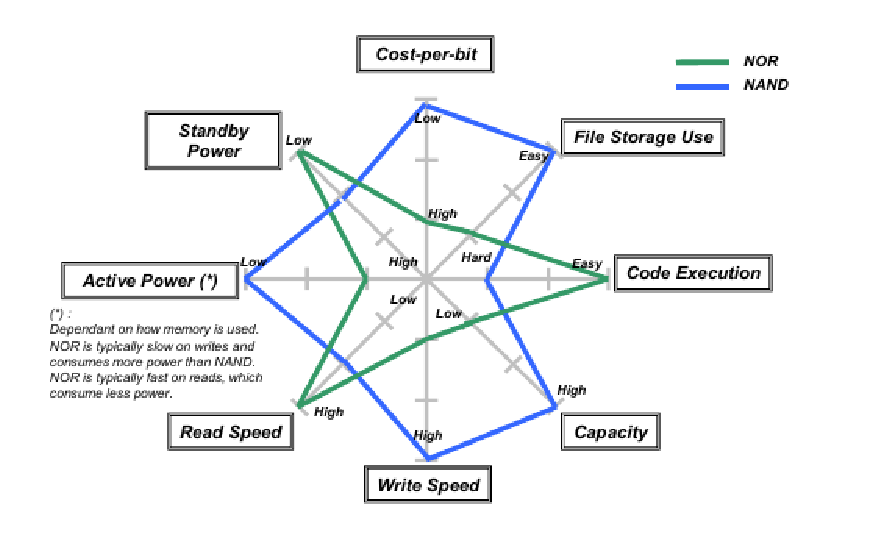
\includegraphics[width=0.60\textwidth,natwidth=610,natheight=642]{fig/comparacionNORNAN}
	\caption{\emph{Diferencia entre Flash NOR y NAND}}
\end{figure}


%------------------------------------------------------------
%          Bibliografia
%------------------------------------------------------------
\bibliographystyle{abbrv}
\bibliography{bsample}
%-------------------------------------------------------------

\end{document}
